% Title: gl2ps_renderer figure
% Creator: GL2PS 1.4.0, (C) 1999-2017 C. Geuzaine
% For: Octave
% CreationDate: Mon Feb 10 16:28:48 2020
\setlength{\unitlength}{1pt}
\begin{picture}(0,0)
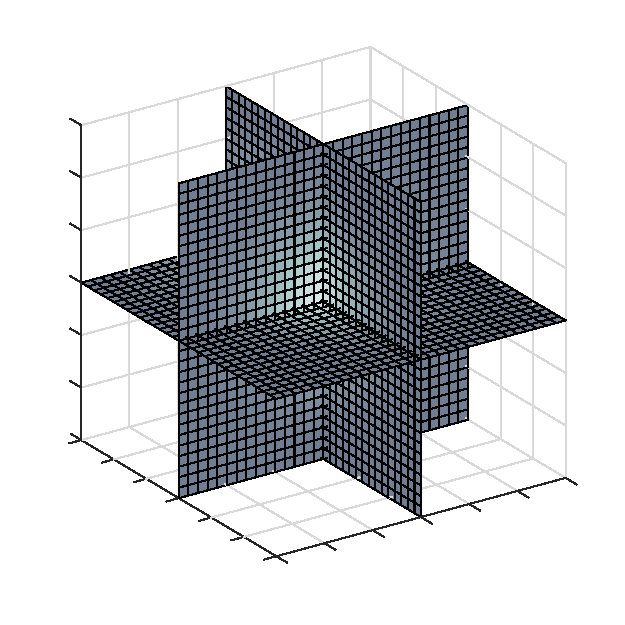
\includegraphics{./img/hw06_slice-inc}
\end{picture}%
\begin{picture}(300,300)(0,0)
\fontsize{10}{0}
\selectfont\put(29.4884,94.4391){\makebox(0,0)[br]{\textcolor[rgb]{0.15,0.15,0.15}{{-3}}}}
\fontsize{10}{0}
\selectfont\put(29.4884,119.623){\makebox(0,0)[br]{\textcolor[rgb]{0.15,0.15,0.15}{{-2}}}}
\fontsize{10}{0}
\selectfont\put(29.4884,144.807){\makebox(0,0)[br]{\textcolor[rgb]{0.15,0.15,0.15}{{-1}}}}
\fontsize{10}{0}
\selectfont\put(29.4884,169.992){\makebox(0,0)[br]{\textcolor[rgb]{0.15,0.15,0.15}{{0}}}}
\fontsize{11}{0}
\selectfont\put(15.4884,169.992){\rotatebox{90}{\makebox(0,0)[b]{\textcolor[rgb]{0.15,0.15,0.15}{{$z$}}}}}
\fontsize{10}{0}
\selectfont\put(29.4884,195.176){\makebox(0,0)[br]{\textcolor[rgb]{0.15,0.15,0.15}{{1}}}}
\fontsize{10}{0}
\selectfont\put(29.4884,220.36){\makebox(0,0)[br]{\textcolor[rgb]{0.15,0.15,0.15}{{2}}}}
\fontsize{10}{0}
\selectfont\put(29.4884,245.544){\makebox(0,0)[br]{\textcolor[rgb]{0.15,0.15,0.15}{{3}}}}
\fontsize{11}{0}
\selectfont\put(61.1193,44.9861){\makebox(0,0)[tr]{\textcolor[rgb]{0.15,0.15,0.15}{{$y$}}}}
\fontsize{10}{0}
\selectfont\put(59.5104,67.2819){\makebox(0,0)[tr]{\textcolor[rgb]{0.15,0.15,0.15}{{1}}}}
\fontsize{10}{0}
\selectfont\put(43.9015,76.5777){\makebox(0,0)[tr]{\textcolor[rgb]{0.15,0.15,0.15}{{2}}}}
\fontsize{10}{0}
\selectfont\put(28.2927,85.8734){\makebox(0,0)[tr]{\textcolor[rgb]{0.15,0.15,0.15}{{3}}}}
\fontsize{11}{0}
\selectfont\put(225.588,33.1457){\makebox(0,0)[tl]{\textcolor[rgb]{0.15,0.15,0.15}{{$x$}}}}
\fontsize{10}{0}
\selectfont\put(234.729,52.4157){\makebox(0,0)[tl]{\textcolor[rgb]{0.15,0.15,0.15}{{1}}}}
\fontsize{10}{0}
\selectfont\put(257.87,58.6858){\makebox(0,0)[tl]{\textcolor[rgb]{0.15,0.15,0.15}{{2}}}}
\fontsize{10}{0}
\selectfont\put(281.012,64.9559){\makebox(0,0)[tl]{\textcolor[rgb]{0.15,0.15,0.15}{{3}}}}
\fontsize{10}{0}
\selectfont\put(106.337,39.3946){\makebox(0,0)[tr]{\textcolor[rgb]{0.15,0.15,0.15}{{-2}}}}
\fontsize{10}{0}
\selectfont\put(90.7282,48.6904){\makebox(0,0)[tr]{\textcolor[rgb]{0.15,0.15,0.15}{{-1}}}}
\fontsize{10}{0}
\selectfont\put(75.1193,57.9861){\makebox(0,0)[tr]{\textcolor[rgb]{0.15,0.15,0.15}{{0}}}}
\fontsize{10}{0}
\selectfont\put(121.946,30.0988){\makebox(0,0)[tr]{\textcolor[rgb]{0.15,0.15,0.15}{{-3}}}}
\fontsize{10}{0}
\selectfont\put(142.165,27.3354){\makebox(0,0)[tl]{\textcolor[rgb]{0.15,0.15,0.15}{{-3}}}}
\fontsize{10}{0}
\selectfont\put(165.306,33.6055){\makebox(0,0)[tl]{\textcolor[rgb]{0.15,0.15,0.15}{{-2}}}}
\fontsize{10}{0}
\selectfont\put(188.447,39.8756){\makebox(0,0)[tl]{\textcolor[rgb]{0.15,0.15,0.15}{{-1}}}}
\fontsize{10}{0}
\selectfont\put(211.588,46.1457){\makebox(0,0)[tl]{\textcolor[rgb]{0.15,0.15,0.15}{{0}}}}
\fontsize{11}{0}
\selectfont\put(155.25,287.5){\makebox(0,0)[b]{\textcolor[rgb]{0,0,0}{{Cross section view of $P(x, y, z)$}}}}
\end{picture}
